The optimized parameters has shown in table \ref{tb:bestparams}.
According to figure \ref{fig:gamma-flux}, secondary $\gamma$-ray product
from both SPL and BPL model yield a similar product via hadronic collision
in the atmosphere. In order to validate the indirect measurement of CR proton,
comparing with a real observations is mandatory which has shown
in figure \ref{fig:proton-flux}. The normalization of this work is
fitted PAMELA data to roughly scale the incident proton spectrum.

\begin{figure}[h!]
    \centering
    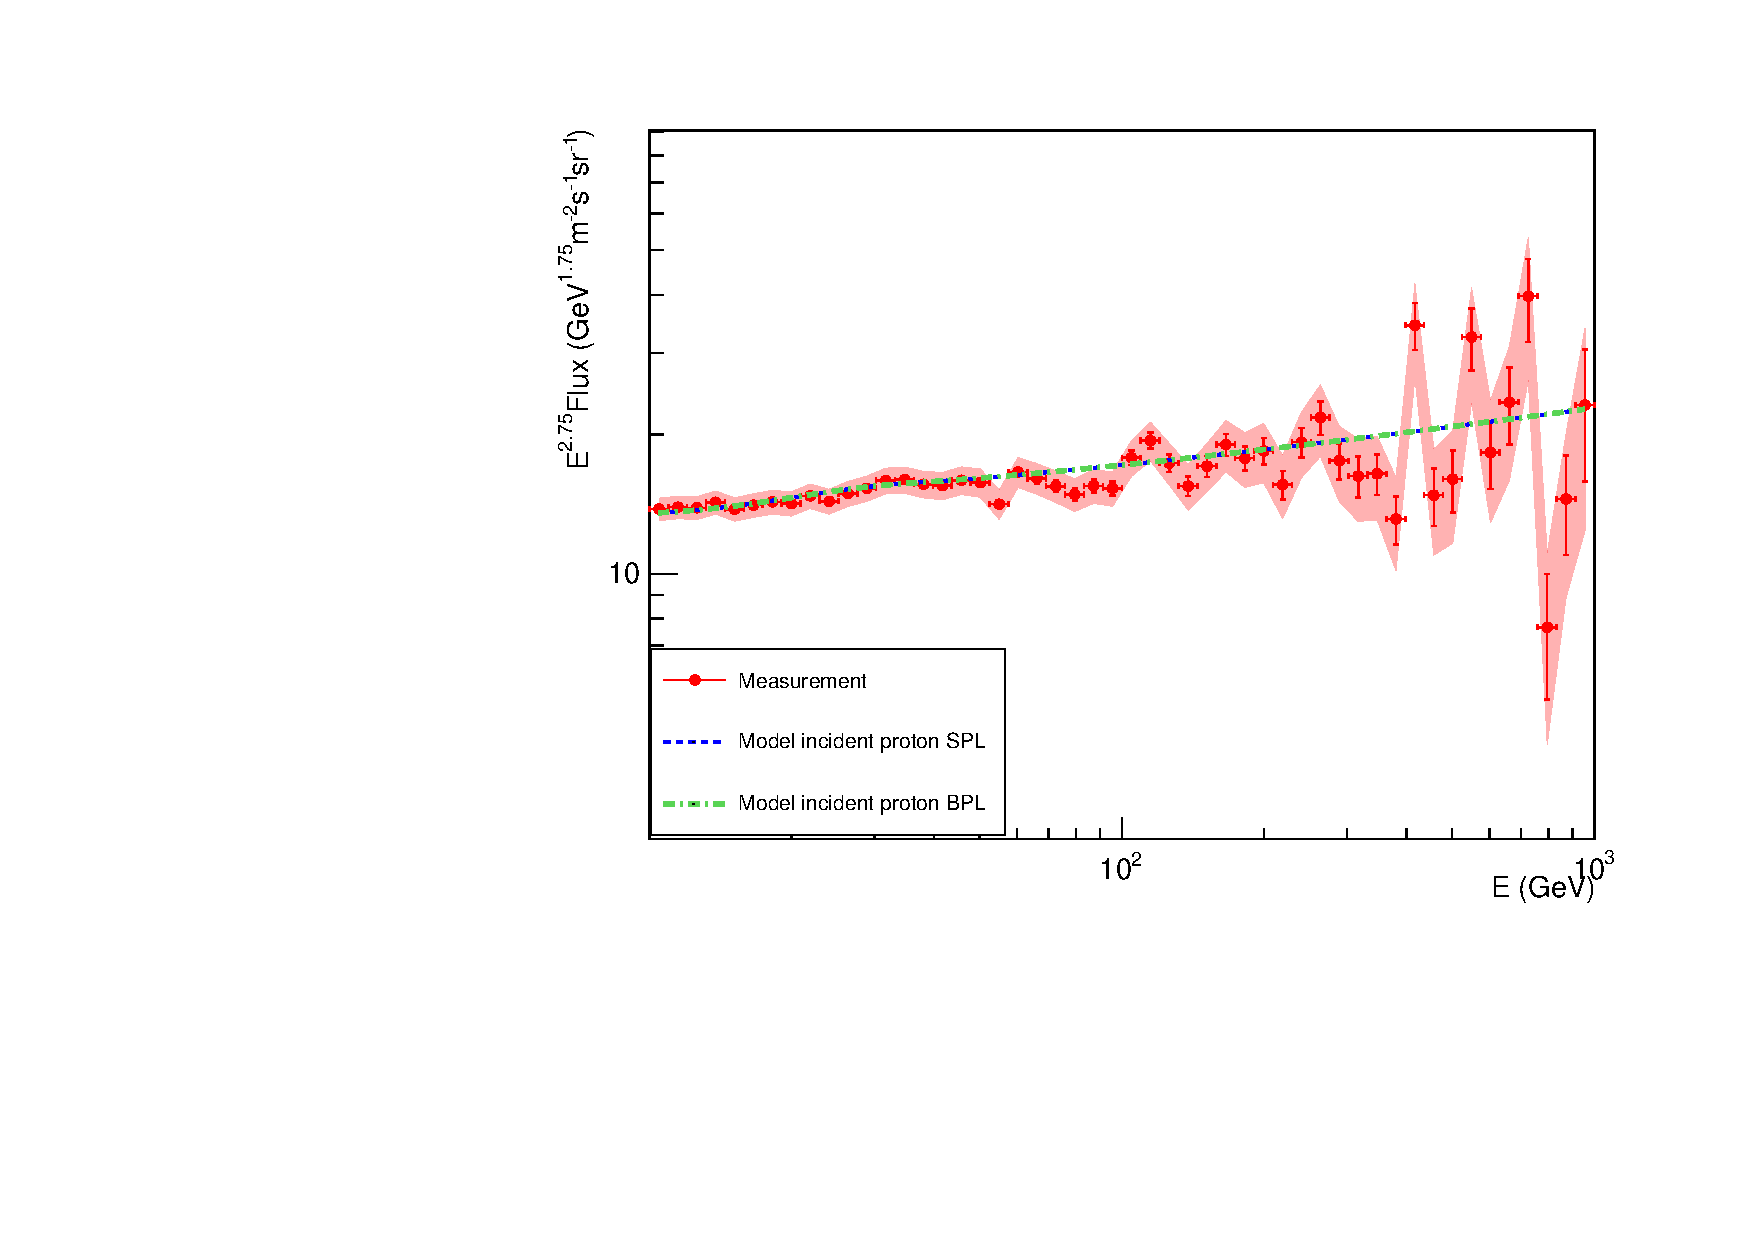
\includegraphics[width=0.7\textwidth]{img/ModelVSMeasurement}
    \caption{Measured $\gamma$-ray flux and the product from incident CRs}
    \label{fig:gamma-flux}
\end{figure}


\begin{center}
\begin{table}[h]
\centering
\caption{Best fitted parameters} 
\label{tb:bestparams}
\begin{tabular}{@{}l*{15}{l}}
\br
Proton CR model&Index 1&Index 2&$E_\text{break}$ (GeV)\\
\mr
SPL&2.70&-&-\\
BPL&2.86&2.63&333\\
\br
\end{tabular}
\end{table}
\end{center}


\begin{figure}[h!]
    \centering
    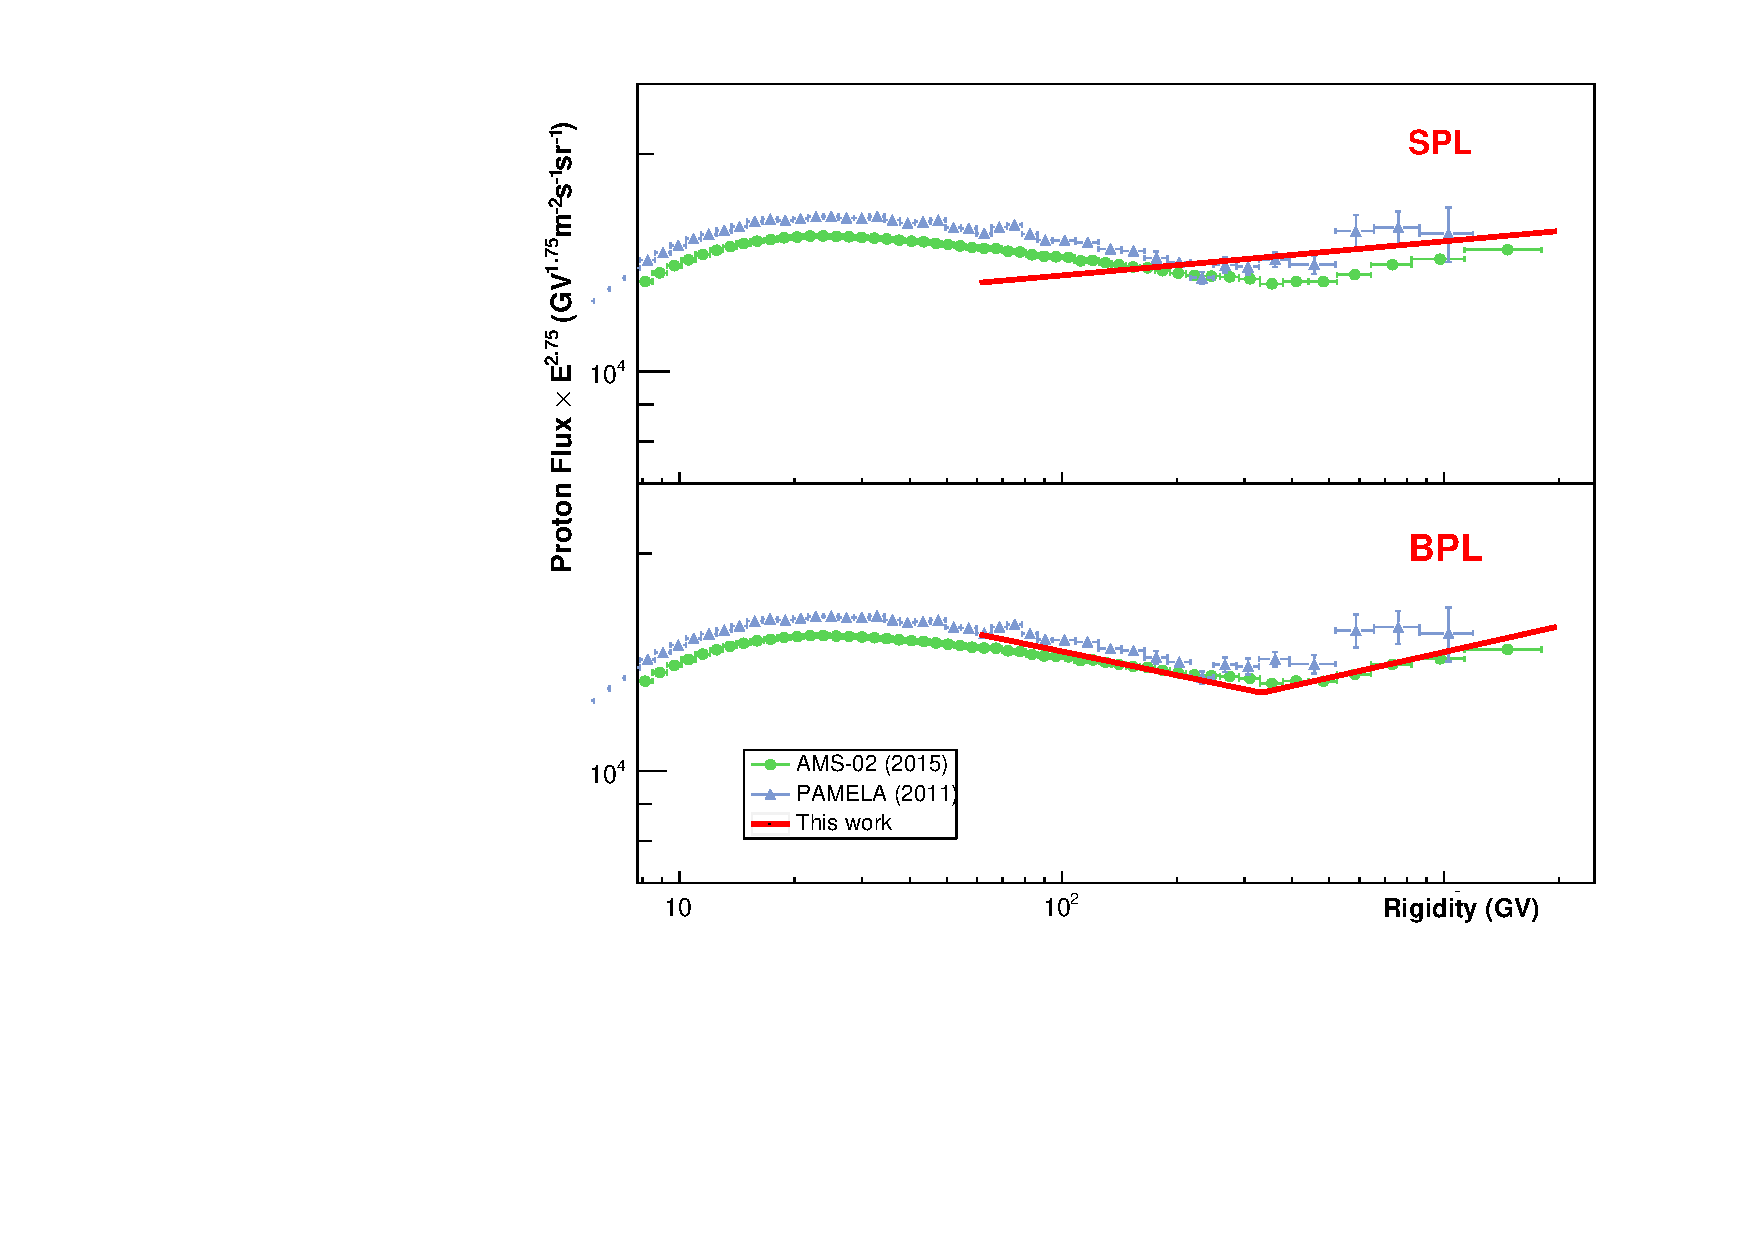
\includegraphics[width=0.8\textwidth]{img/ProtonSpectrumModelMeasurement.pdf}
    \caption{Best fitted proton CRs versus real observations}
    \label{fig:proton-flux}
\end{figure}

